\subsection{The alternating group ($A_n$)}
The alternating group $A_n$ is a very peculiar subgroup of the symmetric group $S_n$. It is 
defined as the group of "even" permutations of $n$ elements. We will see how this group is 
special in many ways. It is the biggest normal subgroup of $S_n$ and this will later turn 
out to be the key of the unsolvibility of the general polynomial equations of degree $n \geq 5$, 
since we will discover that $A_n$ being simple and non-abelian for $n \geq 5$ implies that 
$S_n$ is not Galois-solvable for $n \geq 5$.

\begin{definition}[Even permutation]
    A permutation $\sigma \in S_n$ is called an even-permutation if it can be expressed as a 
    product of an even number of length-2-cycles. 
\end{definition} \vspace{0.2em}

\begin{definition}[Alternating group]
    The set of all even permutations of $S_n$ is called the alternating group and is denoted by
    $A_n$. Since the product of two even permutations is an even permutation, 
    the set $A_n$ is a subgroup of $S_n$. 
\end{definition} \vspace{0.2em}

\begin{definition}[Normal subgroup]
    For every $H$ subgroup of $G$, we say that $H$ is a normal subgroup of $G$, and we indicate it 
    with $H \triangleleft G$ if it's closed under conjugation:

    $$ H \triangleleft G \iff \forall h \in H\;\;\forall g \in G\;\; ghg^{-1} \in H $$
    $$ H \triangleleft G \iff \forall g \in G\;\; gHg^{-1} = H $$
\end{definition} \vspace{0.2em}

\begin{definition}[Central subgroup]
    For every $H$ subgroup of $G$, we say that $H$ is a normal subgroup of $G$, if every 
    element of $G$ commutes with every element of $H$:

    $$ H \texttt{ is central for } G \iff \forall h \in H\;\;\forall g \in G\;\; gh = hg $$
\end{definition} \vspace{0.2em}

\begin{lemma}
    \label{lem:central-subgroup}
    If $H$ is a central subgroup of $G$, then $H$ is also a normal subgroup of $G$.
\end{lemma}
\begin{proof}
    Let $H$ be a central subgroup of $G$. Then, for every $h \in H$ and $g \in G$, we have that 
    $gh = hg$, so we can use that property togheter with the definition of normality to show 
    that $ghg^{-1} = h$, hence it is indeed a normal subgroup:

    $$ ghg^{-1} = g(hg^{-1}) = (gh)g^{-1} = h(g^{-1}g) = h $$
    $$ \therefore\;\; ghg^{-1} \in H \Rightarrow H \triangleleft G $$
\end{proof} \vspace{0.2em}

\begin{lemma}
    The alternating group $A_n$ is non-abelian for $n \geq 4$.
\end{lemma}
\begin{proof}
    We can exibit an example of two even permutations that do not commute in $A_4$, 
    for example the permutations $(1,2)(3,4)$ and $(1,3)(2,4)$. Since these permutations 
    will also be in $A_n$ for every $n \geq 4$, we can conclude that $A_n$ is non-abelian for
    $n \geq 4$. \\
\end{proof} \vspace{0.2em}

\newpage

\begin{lemma}
    The inverse of a permutation preserves the parity of the permutation. In other words, if $\sigma$ is an even
    permutation, then $\sigma^{-1}$ is also an even permutation. The same holds for odd permutations.
\end{lemma}
\begin{proof}
    For every permutation $\sigma \in S_n$, we can write it as a product of length-2-cycles:

    $$ \sigma = (a_1, b_1) \circ (a_2, b_2) \circ \cdots \circ (a_{k-1}, b_{k-1}) 
    \circ (a_{k}, b_{k}) $$
    \vspace{0.2em}
    
    We can then take the inverse of $\sigma$. We can represent the inverse of a
    permutation as the product of the inverses of the length-2-cycles in opposite order:

    $$ \sigma^{-1} = (a_{k}, b_{k})^{-1} \circ (a_{k-1}, b_{k-1})^{-1} \circ \cdots 
    \circ (a_2, b_2)^{-1} \circ (a_1, b_1)^{-1} $$
    \vspace{0.2em}

    This means that the inverse of any permutation has the same number of length-2-cycles prime factors as the 
    original permutation. Since the number of length-2-cycles is even for even permutations and odd for odd permutations,
    we can conclude that the inverse of an even permutation is also an even permutation, and the same holds for odd permutations. \\
\end{proof} \vspace{0.2em}

\begin{lemma}
    The alternating group $A_n$ is a normal subgroup of $S_n$.
\end{lemma}
\begin{proof}
    For every $g \in S_n$ and $h \in A_n$, we can write the permutation $g$ as a product of
    $k$ length-2-cycles, while for every $h \in A_n$, we can write it as a product of $2m$ length-2-cycles:

    $$ g = (a_1, b_1) \circ (a_2, b_2) \circ \cdots \circ (a_{k-1}, b_{k-1}) 
    \circ (a_{k}, b_{k}) $$
    $$ h = (x_1, y_1) \circ (x_2, y_2) \circ \cdots \circ (x_{2m-1}, y_{2m-1}) 
    \circ (x_{2m}, y_{2m}) $$
    \vspace{0.2em}

    This means that the product $ghg^{-1}$ can be written as the product of $k + 2m + k$ 
    length-2-cycles, which is an even number, hence $ghg^{-1}$ is an even permutation. Since 
    $ghg^{-1}$ is an even permutation, we can conclude that $ghg^{-1} \in A_n$. This means that
    $A_n$ is closed under conjugation, hence it is a normal subgroup of $S_n$. \\
\end{proof} \vspace{0.2em}

\newpage

\begin{lemma}
    As a consequence of lemma \ref{lem:central-subgroup}, we can say that if $G$ is abelian, every 
    subgroup of $G$ is a also abelian, hence it is central, and therefore it is also a normal.
\end{lemma} \vspace{0.2em}

Notice that normality doesn't imply centrality, and here is a counter example, Consider 
the permutation $(1,2)(3,4)$ which is even therefore it is in $A_4$. The following 
diagrams makes it clear that the permutation $(1,2)(3,4)$ does not commute with the 
permutation $(2,3)$ with respect to the operation of composition. \\

\begin{figure}[H]
    \centering
    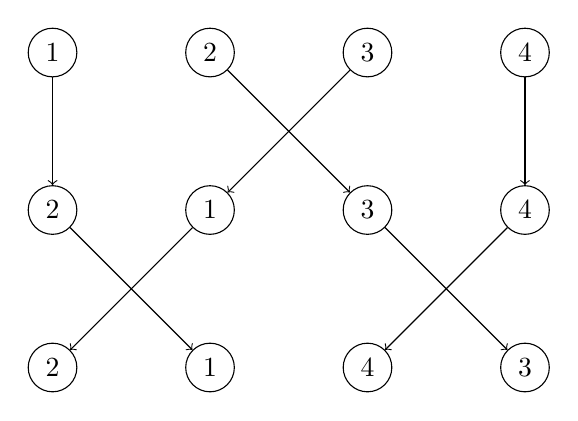
\begin{tikzpicture}
        
        \node (1-1) at (0, 0) [circle, draw] {1};
        \node (1-2) at (2, 0) [circle, draw] {2};
        \node (1-3) at (4, 0) [circle, draw] {3};
        \node (1-4) at (6, 0) [circle, draw] {4};
        
        \node (2-1) at (0, -2) [circle, draw] {2};
        \node (2-2) at (2, -2) [circle, draw] {1};
        \node (2-3) at (4, -2) [circle, draw] {3};
        \node (2-4) at (6, -2) [circle, draw] {4};

        
        \node (3-1) at (0, -4) [circle, draw] {2};
        \node (3-2) at (2, -4) [circle, draw] {1};
        \node (3-3) at (4, -4) [circle, draw] {4};
        \node (3-4) at (6, -4) [circle, draw] {3};

        \draw[->] (1-2) -- (2-3);
        \draw[->] (1-3) -- (2-2); 

        \draw[->] (1-1) -- (2-1);
        \draw[->] (1-4) -- (2-4); 

        
        \draw[->] (2-1) -- (3-2);
        \draw[->] (2-2) -- (3-1); 
        
        \draw[->] (2-3) -- (3-4);
        \draw[->] (2-4) -- (3-3); 

    \end{tikzpicture}
    \caption{The permutation $(2,3) \circ [(1,2)(3,4)]$ }
\end{figure}

\begin{figure}[H]
    \centering
    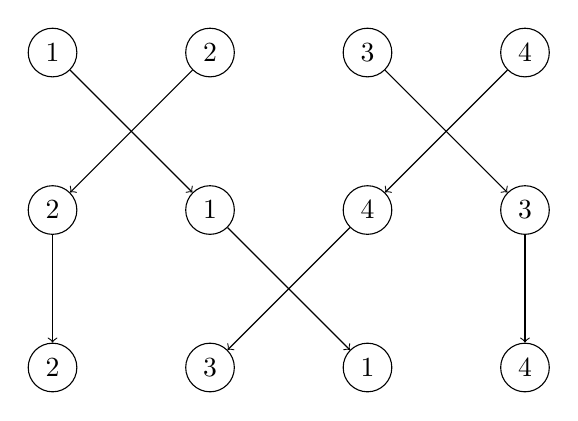
\begin{tikzpicture}
        
        \node (1-1) at (0, 0) [circle, draw] {1};
        \node (1-2) at (2, 0) [circle, draw] {2};
        \node (1-3) at (4, 0) [circle, draw] {3};
        \node (1-4) at (6, 0) [circle, draw] {4};
        
        \node (2-1) at (0, -2) [circle, draw] {2};
        \node (2-2) at (2, -2) [circle, draw] {1};
        \node (2-3) at (4, -2) [circle, draw] {4};
        \node (2-4) at (6, -2) [circle, draw] {3};

        
        \node (3-1) at (0, -4) [circle, draw] {2};
        \node (3-2) at (2, -4) [circle, draw] {3};
        \node (3-3) at (4, -4) [circle, draw] {1};
        \node (3-4) at (6, -4) [circle, draw] {4};

        \draw[->] (1-1) -- (2-2);
        \draw[->] (1-2) -- (2-1); 

        \draw[->] (1-3) -- (2-4);
        \draw[->] (1-4) -- (2-3); 

        
        \draw[->] (2-1) -- (3-1);
        \draw[->] (2-4) -- (3-4); 
        
        \draw[->] (2-2) -- (3-3);
        \draw[->] (2-3) -- (3-2); 

    \end{tikzpicture}
    \caption{The permutation $[(1,2)(3,4)] \circ (2,3)$ }

\end{figure}

This is the case because the requirement of being a normal subgroup is weaker than the
requirement of being a central subgroup. In fact, we can see that the definition of 
centrality implies that $ghg^{-1} = h$, while the definition of normality only requires that
$ghg^{-1} = h' \in H$. So, if $H$ is not central, it is possible for some permutations in 
$H$ to not commute with some permutations in $G$. In fact $A_4$ is normal and not central. \\

\begin{lemma}
    For every $H$ subgroup of $G$, begin central implies being abelian.
\end{lemma}
\begin{proof}
    Let $H$ be a central subgroup of $G$. Then, write down the definition of centrality:

    $$ H \texttt{ is central for } G \iff \forall h \in H\;\;\forall g \in G\;\; gh = hg $$

    Since $H$ is a subgroup of $G$, we have $H \subseteq G$, so we can restrict the 
    "for all" quantifier to just $H$, turning the definition of centrality into the 
    definition of an abelian group:
\end{proof}

\newpage
